\documentclass[a4paper,11pt]{report}
\usepackage[]{amsmath}
\usepackage[]{physics} % \bra, \ket etc
\usepackage{graphicx} %Pour les figures je crois
\usepackage{hyperref}
\usepackage[
    backend=biber, 
    natbib=true,
    style=numeric,
    sorting=none, %Pour faire apparaitre les refs dans l'ordre
    hyperref=true
]{biblatex} %Imports biblatex package
\addbibresource{Bib_ch3.bib} %Import the bibliography file

\usepackage{amssymb} %quelques symboles dont gtrsim /lesssim
\usepackage{subcaption} % package pour faire des subfigures
\usepackage{multirow} % package pour multirow/multicolumn
\usepackage{booktabs} % package pour top/mid/bottom rule
\usepackage{tcolorbox} % toujours plus de boites
\usepackage{xcolor} % Pour avoir des couleurs dans les équations

\title{}
\begin{document}
\chapter{NV-NV cross-relaxations : the fluctuator model}
In this chapter,...



\section{Experimental observation of NV-NV cross-relaxation}
Before we discuss the theoretical complications related to NV-NV cross-relaxations (CR), let us first show the unambiguous experimental proof of the presence of NV-NV CR with dense NV ensembles ([NV]$\gtrsim$ 1 ppm).
\subsection{NV-NV CR between nonequivalent NV centers}
\label{non_equi_valent_CR}
\begin{figure}[h]
\centering
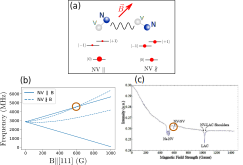
\includegraphics[width=\textwidth]{Figures/NV-NV_non_equivalent}
\caption{label. Taken from \citep{armstrong2010nv}}
\label{non equivalent NV-NV}
\end{figure}
NV-NV CR was first observed more than thirty years ago \citep{holliday1989optical, van1989cross}. The first observations were between non-equivalent NV centers, meaning that the two NV centers involved in the dipole-dipole coupling were not polarized equally.

This scenario can happen for instance when two NV centers from different classes see a different transverse (and longitudinal) magnetic field. Fig \ref{non equivalent NV-NV} illustrates this in the case where the magnetic field is parallel with one of the four classes: $\mathbf{B} \parallel [111]$

When $\mathbf{B} \parallel [111]$, as we discussed in the last chapter, one class sees no transverse field and is therefore always polarized. The three other (equivalent) classes on the other hand get more and more depolarized as the magnetic field amplitude is increased. 

It turns out that there is a co-resonnance at B=592 G between the class parallel to $\mathbf{B}$ and the three other classes. This co-resonance is represented in Fig. \ref{non equivalent NV-NV}-b) by an orange circle.

Fig. \ref{non equivalent NV-NV}-c), which we already saw in the last chapter, shows the change in PL of an ensemble of NV centers as $\mathbf{B}$ is scanned along the [111] axis. For B=592 G, we can see a drop in PL also circled in orange. This drop is the result of the CR between NV centers from the class parallel to $\mathbf{B}$ and NV centers from the three other classes. 

While a difference in polarization is needed to observe a population transfer, it is not enough to explain the drop in PL. This PL drop is due to the difference in brightness between the $\ket{0}$ and $\ket{+1}$ from the different classes involved. The PL contrast between the two states is higher for the class parallel to $\mathbf{B}$ than for the three other ones, which is another consequence of the transverse field.

The co-resonance between two different classes of NV centers with different magnetic field projection is a relatively rare event: it can only occur for the $\ket{0} \to \ket{+1}$ transition, and only for magnetic fields greater than 592 G.

%techniquement y'a les resonances 0->-1 et -1/+1 mais c'est le delbor, j'ai pas envie d'embrouiller plus que ca.

\subsection{NV-NV CR between equivalent NV centers}

\begin{figure}[h]
\centering
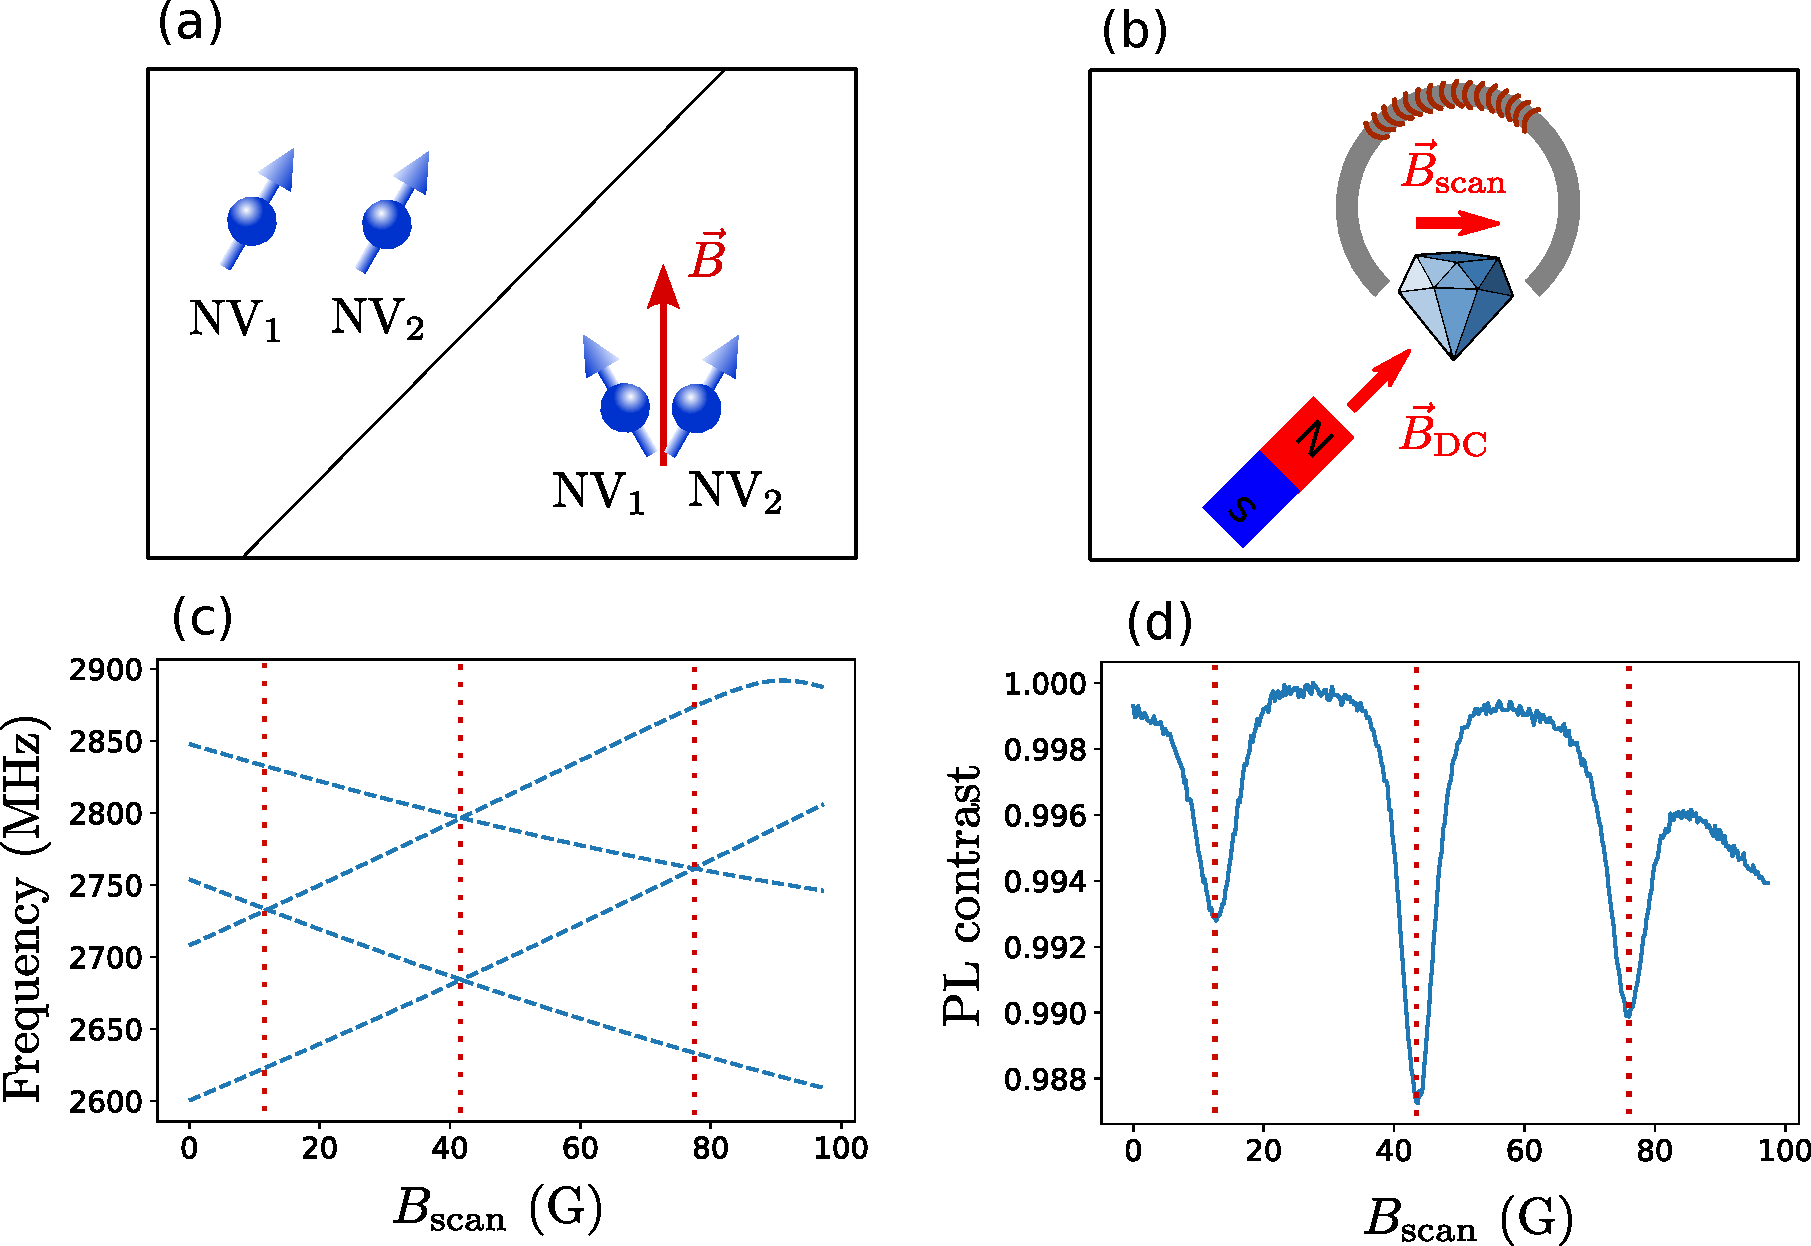
\includegraphics[width=\textwidth]{Figures/NV-NV_equivalent}
\caption{CR between equivalent NV centers for sample ADM-15-1. (a) Representation of equivalent NV centers: either two NVs from the same class, or two classes with the same projected magnetic field. (b) Magnetic setup used for the experiment: a permanent magnet is used to apply a bias magnetic field, and an electromagnet is used to add a variable magnetic field. (c) Simulation of the $\ket{0}\to\ket{-1}$ transition for the 4 classes of NV centers as a function of the scanned magnetic field. The transitions were computed based on several ODMR spectra. The red dotted lines correspond to inter-class resonance (d) Change in the PL of the NV centers ensemble as a function of the scanned magnetic field. The inter-class resonances are reported here.}
\label{equivalent NV-NV}
\end{figure}

More recently, experiments \citep{jarmola2012temperature, mrozek2015longitudinal, choi2017depolarization} on dense NV ensemble ($[\rm NV ] >1\ \rm ppm$) or at low temperature have shown that there was CR even between equivalent NV centers.

I refer by equivalent NV centers to NV centers with the same spin Hamiltonian. This means either NV center from the same class, or NV centers from different classes with the same projection of the magnetic field along their axis. Equivalent NV centers are by nature resonant with each other, and therefore susceptible to CR.

Fig. \ref{equivalent NV-NV} shows an experimental observation of equivalent NV-NV Cr. The key to observe NV-NV CR is to bring some NV centers in and out of resonance with other NV centers, which we can do with the different NV classes. To do so, we need to add an initial bias magnetic field in addition to the scanned magnetic field, as represented in Fig. \ref{equivalent NV-NV}-b). %When doing so, the magnetic field felt by the diamond won't have a fixed orientation during the scan, and when the magnetic field crosses certain crystalline planes (detailed below), its projection on two or more classes of NV centers will be the same.

Fig. \ref{equivalent NV-NV}-c) shows the transition frequencies of the $\ket{0}\to\ket{-1}$ transition for the 4 classes of NV centers on sample ADM-15-1, an HPHT micro-diamond with $[\rm NV]\sim 3\ \rm ppm$. There are three magnetic field values $B_{\rm scan} \sim$ 12, 42 and 77 G for which there is an inter-class resonance. Each of these resonances correspond to a "geometric" resonance where the $B$ field is in a symmetry plane between the two classes, meaning that the two resonant NV classes are indeed equivalent.

Finally, Fig. \ref{equivalent NV-NV}-d) shows the PL contrast as the electromagnet field is scanned. There are 3 very clear dips when $B_{\rm scan} \sim$ 12, 42 and 77 G which coincide with inter-class resonances. We will see later that this PL dip is associated with a decrease of the NV centers spin $T_1$ time from both classes.

This observation, and similar ones done by many groups, seem to indicate that there are CR between equivalent NV centers. This is however incompatible with our previous assumptions that equivalent NV centers are equally polarized and bright. To understand this phenomenon, we will need to introduce new hypotheses.

\section{NV inhomogeneity and the fluctuator model}

\subsection{CR in an inhomogeneous NV bath}
\begin{figure}[h]
\centering
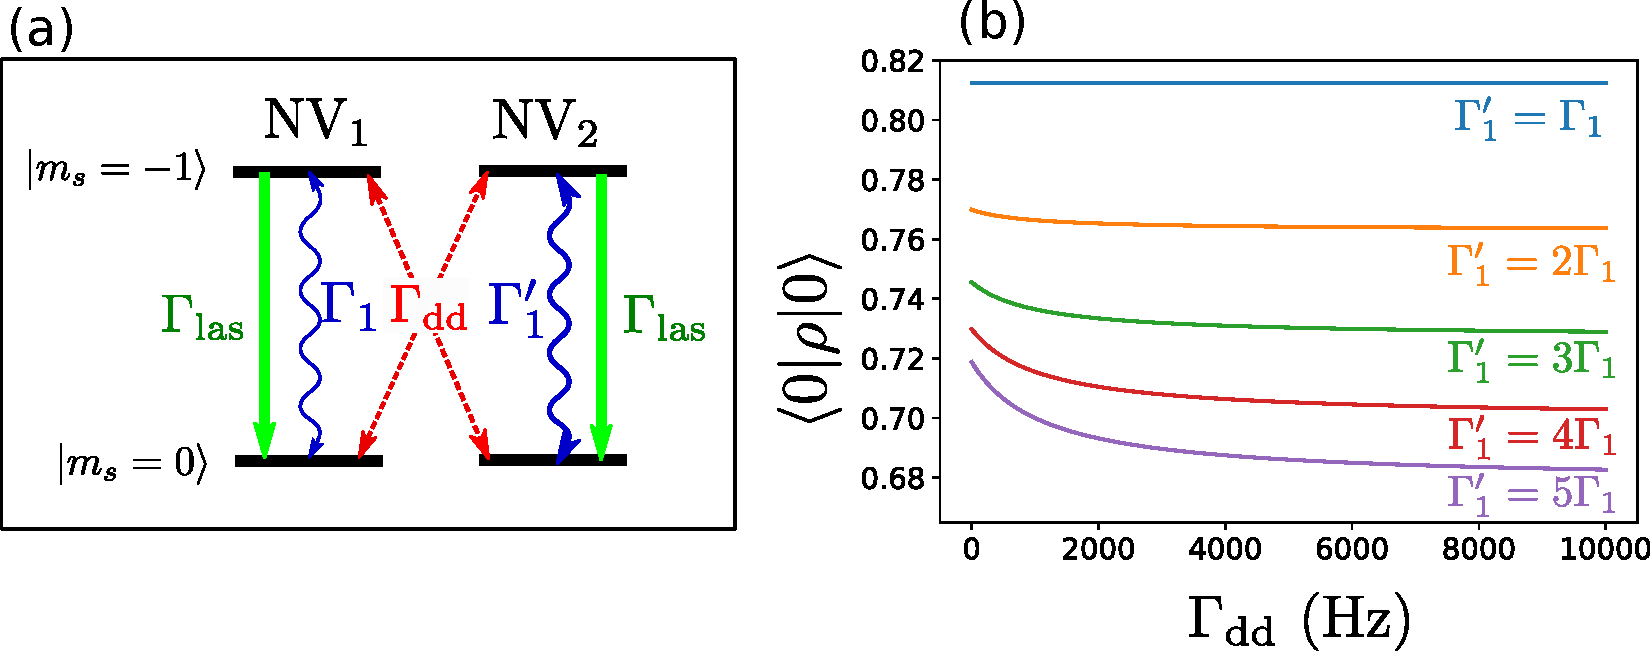
\includegraphics[width=\textwidth]{Figures/inhomogene_2_spins}
\caption{label}
\label{inhomogene}
\end{figure}
A likely explanation to the observed NV-NV CR is that the NV centers are not all equivalents.

Indeed, if we assume that, for instance, the relaxation rate $\Gamma_1=1/T_1$ is not strictly the same for each NV centers, but instead follows a certain distribution $\rho(\Gamma_1)$, then CR between NV centers with different $\Gamma_1$ can explain the observations in Fig. \ref{equivalent NV-NV}.

Fig. \ref{inhomogene} illustrates this case. We are assuming here a coupling between two NV centers with respective relaxation rate $\Gamma_1$ and $\Gamma_1^*$. Fig. \ref{equivalent NV-NV}-a) illustrates the model I chose for this system: $\Gamma_{\rm las}$ represent the optical pumping rate from the $\ket{+1}$ to the $\ket{0}$ state, and $\Gamma_{\rm dd}$ the flip-flop rate between the two spins. I consider here only the incoherent dynamics of the population which I model with various rates. I also only consider the $\ket{0}$ and $\ket{+1}$ states as the results would be the same for the $\ket{0}$ and $\ket{-1}$ states. 

By finding the steady state of these rate equations, I can compute the final population in the $\ket{0}$ for both spins, which I will assume be proportional to the total PL. Fig. \ref{inhomogene}-b) shows this $\ket{0}$ population as a function of the flip-flop rate $\Gamma_{\rm dd}$ for various values of $\Gamma_1^*$.

We can see that when $\Gamma_1^*=\Gamma_1$, as expected, the PL is not modified by the coupling of the two spins regardless of the coupling strength. When $\Gamma_1^*>\Gamma_1$ however, not only is the starting PL slightly lower since NV$_2$ is less polarized, but the PL now decreases as we increase the coupling strength. This effect, which is the origin of the CR contrast, is stronger when the difference between $\Gamma_1$ and $\Gamma_1^*$ is higher.

\subsection{Presentation of the fluctuator model}
Choi et al. in \citep{choi2017depolarization} take this approach a step further by separating the NV centers into two groups: "normal" NV centers with a phonon-limited lifetime outside of dipole-dipole interaction, and "fluctuators" which are NV centers with an intrinsic, extremely fast relaxation mechanism. We are assuming that the fluctuator relaxation rate, $\gamma_f$ is much greater than the optical pumping rate $\Gamma_{\rm las}$. The fluctuators are therefore unpolarized and effectively act as dark spins, similarly to what we discussed in the last chapter.

We should note here that, while this simplifications seem a bit extreme, the fluctuator model is more than a toy model. There are actually good evidence of the presence of these dark NV centers in dense NV ensemble, as will be discussed below.

We will consider the fluctuators act as a Markovian bath, meaning that the fluctuator density matrix will always read $\rho = \frac{1}{3} I$, regardless of its interaction with NV centers. With this assumption, we can compute the modification caused by the fluctuators on the rest of the NV lifetimes.

Other possibilities for the dipole-dipole dependent relaxation rate were considered, such as spin diffusion to non-polarized NV centers (outside of the laser spot) or superradiance, but they were not considered to be viable explanations \citep{choi2017depolarization}
%\begin{pmatrix}
%0.33&0&0 \\
%0&0.33&0 \\
%0&0&0.33
%\end{pmatrix}

\subsection{Single NV center coupled to a single fluctuator}
We will follow here the notations and calculation steps in \citep{choi2017depolarization}. To compute the depolarization induced by the fluctuator bath the NV centers, we should first consider the interaction between a single NV center and a fluctuator. Since we assume the fluctuators to be always depolarized, this step is similar to the coupling of an NV center to a dark spin done in the last chapter.

We will first decompose the dipole-dipole Hamiltonian in a radial and angular part:
\begin{equation}
\mathcal{H}_{\rm dd} \approx - \frac{J_0}{r^3} \left[(g+ih)(\ket{0,+1}\bra{+1,0}+\ket{0,-1}\bra{-1,0}+qS_z^1 S_z^2 \right] + h.c. ,
\end{equation}
where the expression of $J_0, g, h$ and $q$ is given in appendix [REF]. $g, h$ and $q$ are dimensionless factors that are function of the relative orientation of the two dipoles.

We then introduce the dimensionless number $\eta$ defined as:
\begin{equation}
\eta^2=\frac{1}{3} (\abs{g}^2+\abs{h}^2)  \frac{4\gamma_f^2}{(\omega_f - \omega_{NV})^2+4\gamma_f^2},
\end{equation}
where $\gamma_f=1/T_1^f$ is the fluctuator decay rate. This number $\eta$ encapsulate both the geometry of the problem (trhough $g$ and $h$) and the resonance condition between the NV center and the fluctuator.

Finally, the additional depolarization rate induced by the fluctuator on the NV center reads:
\begin{equation}
\gamma_s(\mathbf{r})=\left(\frac{J_0}{r^3}\right) \frac{\eta^2}{\gamma_f}.
\end{equation}
Compared to eq. [REF], we have replaced here $\Gamma_2^*$ by $\gamma_f$. This is because we assume that the pure dephasing, supposedly equal for the NV center and the flucutator, is smaller than the depolarization rate $\gamma_f$. We will further discuss this hypothesis later.

\subsection{Ensemble of NV centers coupled to a bath of fluctuators}

We now need to compute the average depolarization caused by the ensemble of fluctuators on the ensemble of NV centers.

We consider each fluctuator as in independant depolarization source, therefore the depolarization on a single NV center reads: 
\begin{equation}
\gamma=\sum_i \gamma_s(\mathbf{r}_i).
\end{equation}
We then want to compute the distribution $\rho(\gamma)$ defined as:
\begin{equation}
\rho(\gamma)=\int d\{r_i\} \rho(\{r_i\})\, \delta \left( \sum_i \gamma_s(\mathbf{r}_i) - \gamma \right).
\end{equation}
To do so, we need to determine the distribution of the fluctuators positions $\{r_i\}$. Assuming that they are homogeneously distributed in the bulk of the material, we find:
\begin{equation}
\rho(\gamma)=\frac{e^{-1/(4\gamma T)}}{\sqrt{4\pi \gamma^3 T}},
\end{equation}
where the time constant $T$ was introduced and is defined as:
\begin{equation}
\frac{1}{T}=\left(\frac{4\pi n_fJ_0\bar \eta}{3}\right)^2 \frac{\pi}{\gamma_f},
\label{eq 1/T}
\end{equation}
with $n$ the fluctuator density and $\bar \eta$ the averaged value of $\abs{\eta}$: $\bar \eta = \int \rm{Prob}(\eta) \abs{\eta} d\eta$.

Finally, the polarization dynamics from the ensemble of NV centers can be computed:
\begin{equation}
P(t)=\int_0^\infty \rho(\gamma)\, e^{-\gamma t}d\gamma= e^{-\sqrt{t/T}}.
\end{equation}

In conclusion, the fluctuators causes a depolarization on the NV ensembles with a timsecale $T$ given by \ref{eq 1/T}, and the dynamics of this depolarization is that of a stretched exponential, unlike the phonon-induced depolarization which is purely exponential. 

It should be noted that the stretched exponential nature of the decay is not proper to the fluctuator model. \citep{hall2016detection} came to the same conclusion by analyzing the resonant coupling of NV centers with a P1 bath. The stretched exponential is a result from localized noise sources, randomly distributed in the bulk (3D).

\subsection{Possible microscopic origin of the fluctuators}

We should note first that a similar problem of spin ensemble relaxation rate increasing with the spin concentration was observed more than six decades ago with phosphorus doped silicon \citep{feher1959electron,honig1960electron}. It was proposed that the cause of the relaxation was the presence of fast relaxing centers coupled to the slow relaxing centers through spin diffusion \citep{honig1960electron, sugihara1963spin, yang1968concentration, vugmeister1978spin, berman2005spin}. 

This conclusion is based on previous observations on the relaxation of nuclear spins \citep{bloembergen1949interaction, de1958relaxation, blumberg1960nuclear}, where some nuclear spins had a considerably reduced lifetime due to their proximity to paramagnetic ions, and the resonant energy transfer between molecules \citep{forster1949experimentelle, eisenthal1964influence, yokota1967effects}, where excited donor molecules are coupled through dipole-dipole interaction to non-excited acceptors, and where the stretched exponential dynamics of the donors was first observed \citep{forster1949experimentelle}.

In the case of P-doped Si, the origin of the fast relaxing centers is thought to be closely packed P impurities, so that the electronic wavefunctions of (at least) two P centers overlap. In that case two phenomena occur: the possibility of electron tunneling, and the apparition of a contact interaction term in the dipole-dipole Hamiltonian (see appendix [REF]). Both of these phenomena could lead to fast spin relaxation, the tunneling because the spin hopping is accompanied by a spin reversal \citep{sugihara1963spin}, and the modulation of the contact interaction strength $J$ by the crystal phonons \citep{honig1960electron}. Technically, the non-contact dipole-dipole interaction is also modulated by the phonons, but the effect is too small to account for the fast depolarization.

Similarly, \citep{choi2017depolarization} suggests that the origin of fluctuators in NV centers are closely packed NV centers or NV-impurity pairs which undergo rapid electron hopping and spin depolarization. To prove their point, they look at the charge dynamics in their sample and find that there is charge recombination in the dark with a corresponding tunneling rate $\sim 10\ \rm ns$. In contrast to P-doped Si, the NV centers are not the most abundant electronic defects in the crystal, this is why the NV$^--$N$^+$ pair in particular is thought to be a likely candidate for the fluctuators \citep{manson2018nv}.

\section{Experimental investigation of the fluctuator model}
We will now show experimental results related to the predictions of the fluctuator model.
\subsection{The stretched exponential lifetime}
\begin{figure}[h]
\centering
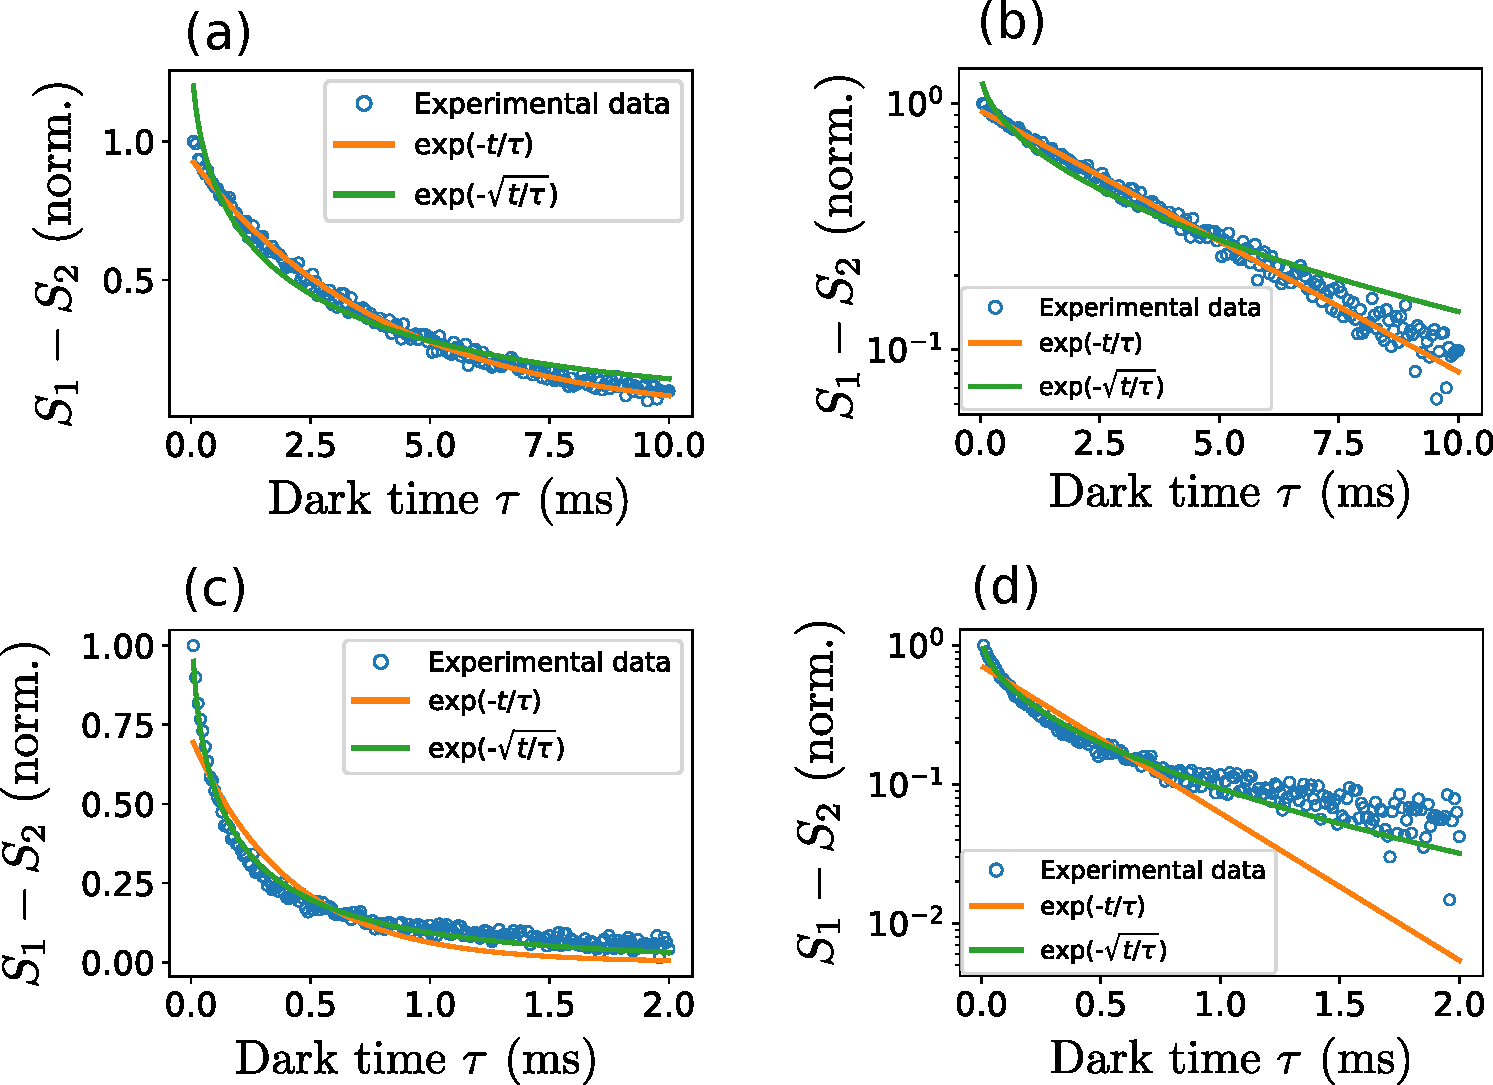
\includegraphics[width=\textwidth]{Figures/Stretch_vs_pas_stretch}
\caption{T1 measurement following the protocol described in [REF]. The best exponential and stretched exponential fits are given each time. a) Sample ADM-15-2 with B=0. The optimal $T_1$ values are $T_1^{\rm stretch}=150\ \mu \rm s$ and $T_1^{\rm exp}=410\ \mu \rm s$. b) Sample CVD-pink with B$\neq$0 and a single class probed. The optimal $T_1$ values are $T_1^{\rm stretch}=1.9\ \rm ms$ and $T_1^{\rm exp}=4.1\ \rm ms$}
\label{stretch_or_not_stretch}
\end{figure}
$T_1$ measurements with dense ensemble of NV centers and when many classes are resonant with each other (typically when B=0) indeed tend to show stretched exponential profiles.

Fig. \ref{stretch_or_not_stretch} shows an example of that: in Fig. \ref{stretch_or_not_stretch}-a) the $T_1$ measurement comes from sample ADM-15-2 at B=0. The profile is clearly better fitted by a stretched exponential than a regular exponential, and the timescale found $T_1^{\rm stretch}=150\ \mu \rm s$ is much shorter than the expected phonon limite lifetime of a few ms.

On the other hand, Fig. \ref{stretch_or_not_stretch}-b) shows a $T_1$ measurement coming from sample CVD-pink for B$\neq$0. This time the profile is more exponential, and the value $T_1^{\rm exp}=4.1\ \rm ms$ is coherent with a phonon-limited lifetime. Even though CVD-pink shows some NV-NV CR feature, the spin dynamics in this sample is still dominated by the phonons, which explains the exponential profile.


\subsection{Fitting $T_1$ profile in the general case}

\begin{figure}[h]
\centering
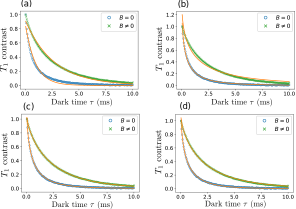
\includegraphics[width=\textwidth]{Figures/various_fit_formulae}
\caption{Different fitting procedure on two $T_1$ measurements done on sample ADM-150-1 for $B=0$ and $B\neq0$. \\ a) Exponential fit $S(\tau)=\exp (-\tau/T_1^{\rm ph})$. \\ b) Stretched exponential fit $S(\tau)=\exp (-\sqrt{\tau/T_1^{\rm dd}})$. \\ c) Bi-exponential fit $S(\tau)=\exp (-\tau/T_1^{\rm ph} -\sqrt{\tau/T_1^{\rm dd}})$. \\ d) Bi-exponential fit with fixed $T_1^{\rm ph}=5\ \rm ms$: $S(\tau)=\exp (-\tau/5 -\sqrt{\tau/T_1^{\rm dd}})$.}
\label{various_fit_formulae}
\end{figure}

\begin{table}[htbp]
\centering
\caption{Fitting parameters for Fig.
 \ref{various_fit_formulae}}
 \label{fitting table}
\begin{tabular}{c|cc|cc}
\toprule
Figure &  \multicolumn{2}{c}{$B=0$} & \multicolumn{2}{c}{$B\neq0$}\\
\midrule
{} &  $T_1^{\rm ph}$ (ms)& $T_1^{\rm dd}$ (ms)&  $T_1^{\rm ph}$ (ms)& $T_1^{\rm dd}$(ms)\\
Fig. a) & 0.95 & * & 2.64 & * \\
Fig. b) & * & 0.32 & * & 1.03  \\
Fig. c) & 6.75 & 0.44 & 4.22 & 7.19 \\
Fig. d) & \textbf{5} & 0.51 & \textbf{5} & 4.65 \\
\bottomrule
\end{tabular}

Bold characters indicate parameters that were arbitrarily fixed.
  
\end{table}

For many samples however, the $T_1$ profile is neither fully exponential nor fully stretched exponential, because the relaxation time associated with CR, which we will call $T_1^{\rm dd}$ is of the same order as the phonon limited lifetime $T_1^{\rm ph}$. Sometimes the same sample can go from mostly exponential to mostly stretched exponential depending on the number of NV-NV co-resonances, forcing us to include both aspects if we want a unique fitting formula.

Fig. \ref{various_fit_formulae} shows four different fitting procedure on the two same measurements. The measurements here are two $T_1$ measurements done on the same sample ADM-150-1, following the protocol described in [REF], with and without an external magnetic field ($\sim 50 G$). The magnetic field was strong enough to split the four classes and only one class was probed in the case $B\neq0$ , whereas all 4 classes were resonant in the case $B=0$, which strongly increases the NV-NV CR. 

The fits used here are either purely exponential or purely stretched exponential, or a combination of both where the exponential lifetime $T_1^{\rm ph}$ was either left as a free parameter or fixed at a value $T_1^{\rm ph}=5\ \rm ms$. The values of the different fitting parameters used is reported in Table \ref{fitting table}.

We can see that neither the purely exponential nor stretched exponential fits can be satisfying for both measurements: the $B=0$ curve is poorly fitted by the exponential fit and the $B \neq 0$ curve is poorly fitted by the stretched exponential. The protocols that include both exponential and stretched lifetimes correctly fit both curves. In the case of Fig. \ref{various_fit_formulae}-d), we arbitrarily fixed $T_1^{\rm ph}=5\ \rm ms$ since this is the value we typically measure on samples with low NV density, and we expect that the phonon-limited exponential lifetime is not modified by the NV concentration.

Since the protocol where $T_1^{\rm ph}$ was fixed and the one where it wasn't both correctly fit our data, we decided to use the protocol where $T_1^{\rm ph}$ was fixed because there is one less free parameter in the fitting function, and the values we obtain on $T_1^{\rm dd}$ can be directly compared. 

We should note however that the values of $T_1^{\rm dd}$ we obtain are not absolute. Indeed, in the case of Fig. \ref{various_fit_formulae}, the value of $T_1^{\rm ph}$ can be somewhat arbitrarily fixed between 3 and 6 ms with satisfying fits, and the resulting values $T_1^{\rm dd}$ can vary by almost an order of magnitude in the case of $B\neq0$. While this technique of measuring $T_1^{\rm dd}$ is relatively sensitive and reproducible, it is not very accurate.

\begin{figure}[h]
\centering
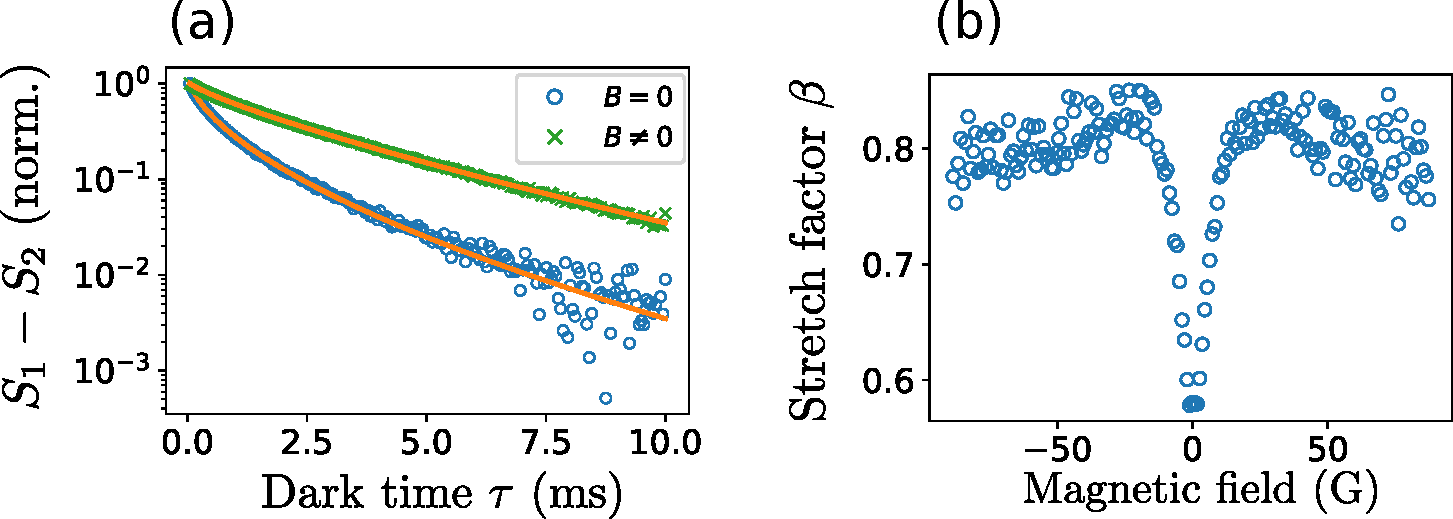
\includegraphics[width=\textwidth]{Figures/betas}
\caption{a) Same two measurements as Fig. \ref{various_fit_formulae} with the fitting formula $S(\tau)=\exp ((-\tau/T_1)^{\beta})$. The fitting parameters are $\beta=0.58$ and $T_1=0.46\ \rm ms$ for $B=0$, and $\beta=0.80$ and $T_1=2.15\ \rm ms$ for $B\neq0$. b) Optimal $\beta$ parameter found for each $T_1$ measurement as a function of the external magnetic field (still on sample ADM-150-1).}
\label{betas}
\end{figure}

Finally, another fitting procedure is shown in Fig. \ref{betas}. This time we are using a single stretched exponential with an arbitrary stretch factor $\beta$. Fig. \ref{betas}-b) shows the optimal $\beta$ parameter as a function of the external magnetic field. We can then confirm that the $T_1$ profile gets closer to a stretched exponential ($\beta=0.5$) when $B$ goes to 0. 

Even though this method also yields satisfying fits, it needs two free parameters to work ($\beta$ and $T_1$), so we decided to go with the method of Fig. \ref{various_fit_formulae}-d) instead.

\subsection{The fluctuators linewidth}

\begin{figure}[h]
\centering
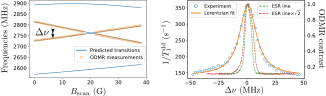
\includegraphics[width=\textwidth]{Figures/fluctuator linewidth}
\caption{Measurement of the fluctuators linewidth using the same setup as in Fig. \ref{equivalent NV-NV}. a) Simulation of the $\ket{0} \to \ket{-1}$ transition frequency for the four classes of NV centers and actual frequencies of the two central classes from ODMR measurements. b) Measurement of $T_1^{\rm dd}$ as a function of the splitting $\Delta \nu$ between the two central classes, fitted with a Lorentzian of half-width $\sigma=8.78\ \rm MHz$. The green dashed line correspond to the ODMR spectrum of a single class of NV centers, and the red dashed one to the same line scaled up by a factor $\sqrt{2}$}
\label{fluct linewidth}
\end{figure}

One of the main arguments in favor of the fluctuator model is the measurement of the fluctuators linewidth. In the model, we assumed that fluctuator's lifetime $T_1^f=1/\gamma_f$ was so short that the fluctuators linewidth was lifetime-limited, whereas the normal NV centers linewidth is limited by the inhomogeneous broadening $T_2^*>T_1^f$.

We can experimentally verify this hypothesis: the fluctuator are effectively dark to ODMR measurement since they are not polarized, but we can measure their linewidth through CR the same way we would do for a dark spin, as detailed in the last chapter.

Fig. \ref{fluct linewidth} shows an experiment similar to the one presented in Fig. \ref{equivalent NV-NV}. A variable magnetic $B_{\rm scan}$ in addition to an offset magnetic field $B_{\rm DC} \sim 100\ \rm G$ are used in order to create a crossing between two classes of NV centers, but this time measuring the spin decay rate instead of the PL.

Fig. \ref{fluct linewidth}-a) shows the simulated transitions of the four classes of NV centers as a function of the magnetic field. Because the $T_1$ measurement protocol described in [REF] requires a resonant microwave pulse with the NV probed, we specifically record ODMR spectra of the two central lines to get a precise measurement of the Larmor frequency. In the region where the two ODMR lines overlap we have to use a linear regression to get the Larmor frequency of each class.

Fig. \ref{fluct linewidth}-b) shows the dipole-dipole induced relaxation rate $T_1^{\rm dd}$ as a function of the detuning $\Delta \nu$ between the two central classes. For each magnetic field value, a $T_1$ profile was recorded and fitted following the procedure described in Fig. \ref{various_fit_formulae}-d) where we again fixed $T_1^{\rm ph}=5\ \rm ms$. We also show the ODMR spectrum of a single NV class for comparison.

We can clearly see that the increase in $T_1^{\rm dd}$ is much broader than the ODMR line of the NV centers, whereas in a standard CR process, we expect the decay rate to be proportional to the spectral overlap of the two classes \citep{hall2016detection}. If we assume that both NV classes spectral response is a gaussian of same width $\sigma$, then the spectral overlap between the two classes is also a gaussian of width $\sqrt{2} \sigma$. Fig. \ref{fluct linewidth}-b) also shows the ODMR line scaled by a factor $\sqrt{2}$, which is still much narrower than the $1/T_1^{\rm dd}$ line.

A potential explanation for the broadening of the $1/T_1^{\rm dd}$ line could be the interaction strength between the NV center and the fluctuator. However, for [NV] $\sim$ 5 ppm, the average dipole-dipole coupling strength between closest NV neighbor is $\expval{\mathcal{H}_{\rm dd}} \sim 46\ \rm kHz$, which cannot explain the $\sim 4\ \rm MHz$ broadening that we observe.

\begin{figure}[h]
\centering
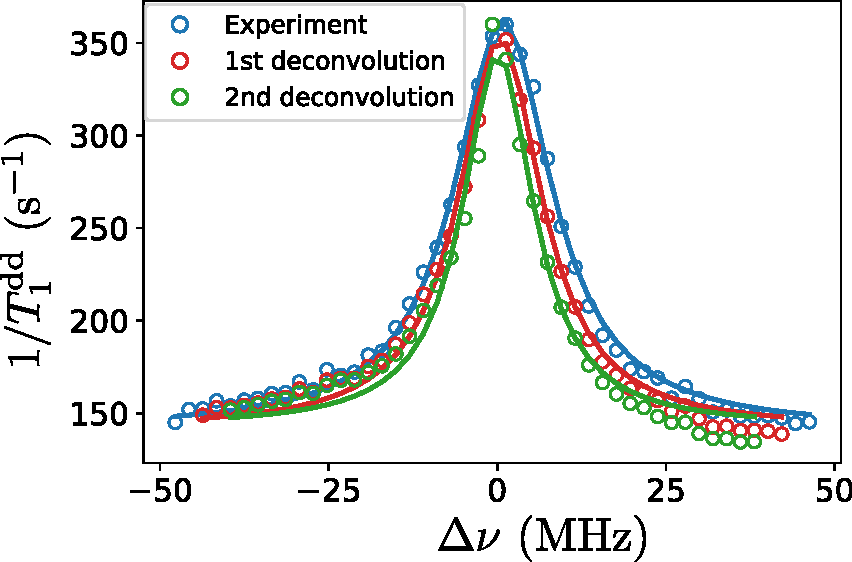
\includegraphics[width=0.6\textwidth]{Figures/deconvolution}
\caption{Blue curve $1/T_1^{\rm dd}$ data presented in Fig. \ref{fluct linewidth}. Red curve: deconvolution of the blue curve the  by the ODMR line shown on the same figure. Green curve: deconvolution of the red curve the  by the ODMR line. All three curves are fitted with Lorentzian of respective half widths 8.78, 7.49 and 6.38 MHz}
\label{deconvolution}
\end{figure}

The fluctuator model provides another explanation: the fluctuator spectral response is broaden by its very short lifetime. This also explains why the $1/T_1^{\rm dd}$ line is well matched by a Lorenzian, while the ODMR lines are closer to Gaussians in our sample. 

We can now extract the fluctuator lifetime from the data in Fig. \ref{fluct linewidth} by taking out the contribution of $T_2^*$ on both the NV and the fluctuator spectral response. 

The first way to do this is to follow the instructions in \citep{hall2016detection} and deconvolve the $1/T_1^{\rm dd}$ data by the ODMR spectrum using a Wiener deconvolution algorithm. The result of the deconvolution is shown in Fig. \ref{deconvolution}: the data is deconvolved once to get the spectral response of the fluctuator (red curve), and a second time to get only the lifetime contribution of the fluctuator (green curve). Fitting with Lorentzians, we find a final value $\Gamma_2 =\frac{\gamma_f}{2} = (2\pi) 6.38\ \rm MHz$ which corresponds to a fluctuator lifetime $T_1^f=\frac{1}{\gamma_f}=12.5\ \rm ns$.

Another, simpler alternative is to consider that the $1/T_1^{\rm dd}$ profile is a Voigt profile given by the convolution of two Gaussians of half width at half maximum (HWHM) $f_G=\sqrt{2 \ln (2)}\sigma$ and a Lorentzian of HWHM $f_L$:
\begin{align*}
\Gamma_1^{\rm dd}&\propto \mathcal{G}(f_G)*(\mathcal{L}(f_L)*\mathcal{G}(f_G)) \\
&\propto \mathcal{L}(f_L)*\mathcal{G}(\sqrt{2} f_G),
\end{align*}
where $\mathcal{G}(f_G)$ and $\mathcal{L}(f_L)$ denote Gaussian and Lorentzian functions of HWHM $f_G$ and $f_L$ respectively.
We can then use the formula of a pseudo-Voigt profile which gives an approximation of the Voigt profile's HWHM $f$ as a function of $f_G$ and $f_L$ \citep{wiki:VoigtProfile}:
\begin{equation}
f = [f_G^5 + 2.69269 f_G^4 f_L + 2.42843 f_G^3 f_L^2 + 4.47163 f_G^2 f_L^3 + 0.07842 f_G f_L^4 + f_L^5]^{1/5}.
\end{equation}

With $f=8.78\ \rm MHz$ and $\sqrt{2}f_G=4.33\ \rm MHz$, I find $f_L=6.54\ \rm MHz$ for a final lifetime value $T_1^f = 12.2\ \rm ns$, a value consistent with the one found with the deconvolution method.

Doing similar calculations, \citep{choi2017depolarization} found $\gamma_f=1/T_1^f=3.3\ \rm MHz$, although given their experimental values - full width at half maximum (FWHM) of 25 MHz for the lifetime profile and 9.3 MHz for the ODMR line - I obtain using my method $\gamma_f= 15.7\ \rm MHz$ and $T_1^f=10.1\ \rm ns$. The main difference comes from the fact that they considered the spectral half-width of the fluctuators to be $2\gamma_f$ whereas I consider it to be $\gamma_f/2$.


\section{Trouver un bon titre}

The main tool to probe NV-NV CR is to use the co-resonances between the NV classes. While it is not possible to completely shut down the CR, because the NV centers from the same class are always resonant with each other, we can tune the density of resonant NV centers (and supposedly resonant fluctuators) by a factor of 4 by playing with the inter-class co-resonances. We will discuss here the various ...

\subsection{Geometric conditions for inter-class resonance}

\begin{figure}[h]
\centering
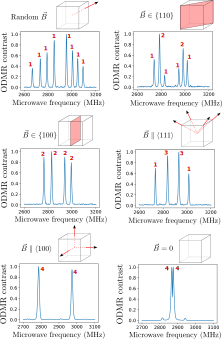
\includegraphics[width=0.8\textwidth]{Figures/Resonance_geometries}
\caption{ODMR spectra on sample ADM-15-3 as a function of the magnetic field orientation. The field amplitude is $\sim 60\ \rm G$. Red numbers represent the number of resonant classes for each ODMR line. The cubes represent the diamond unit cell, and the red planes/arrow the possible orientations of the magnetic field}
\label{ODMR_geometries}
\end{figure}

There are four possibilities to obtain inter-class resonance (outside of the non-equivalent CR discussed in sec. \ref{non_equi_valent_CR}). These possibilities are:
\begin{itemize}
\item $\mathbf{B} \in \{110\}$. We refer by $\{110\}$ as any plane orthogonal to a $\langle 110 \rangle$ or equivalent direction. In this magnetic configuration, two classes are at resonance and the two other ones are spectrally isolated.
\item $\mathbf{B} \in \{100\}$. In this magnetic configuration, the four classes form two pairs of co-resonance.
\item $\mathbf{B} \parallel \langle 111 \rangle$. In this configuration discussed in the last chapter, one class is aligned with the magnetic field and is spectrally isolated while the three other form a resonant triplet.
\item $\mathbf{B} \parallel \langle 100 \rangle$. In this configuration also discussed in the last chapter, the four classes are resonant.
\end{itemize}
We should add to this list the case $\mathbf{B}=0$ where all four classes are also resonant, and any other possibility (which I will call random $\mathbf{B}$) where all four classes are spectrally separated. 

An ODMR spectrum and a representation of the magnetic field in the diamond unit cell for each of these six possibilities is shown in Fig. \ref{ODMR_geometries}.

\begin{figure}[h]
\centering
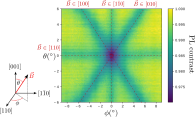
\includegraphics[width=\textwidth]{Figures/carte}
\caption{PL contrast as a function of the magnetic field polar and azimuthal angle with respect to the [100] axis on sample CVD-pink. The field amplitude is $\abs{B} \sim 115 G$. The locus of the magnetic field in specific planes is noted by red dashed lines.}
\label{Carte}
\end{figure}

This relation between NV-NV class resonances and the magnetic field being in specific crystalline planes or directions means that we can determine the crystal main axes simply by PL experiments.

Fig. \ref{Carte} shows a map where we simply monitored the PL of sample CVD-pink while scanning the magnetic field angle around the [001] axis, thanks to a permanent magnet on a motorized goniometer. We have also reported the locus of $\mathbf{B}$ being in the planes [100], [010], [110] and [$1\bar 1 0$].

We know that when $\mathbf{B}$ belongs to any of these four planes, there is a co-resonance between at least two NV classes. This co-resonance leads to an increase in NV-NV CR (or NV-fluctuator CR) and a faster depolarization of the spins involved, which ultimately leads to a drop in PL. We can indeed see in fig. \ref{Carte} that there is clear correlation between the loci of $\mathbf{B}$ and drops in PL. We can also see that the PL is at its lowest when $B\parallel [001]$, which corresponds to a four class degeneracy.

\subsection{$T_1$ dependency on magnetic field}

\section{Limitations of the fluctuator model}
La modification des T1, tjr plus petite que prévue (faire un tableau), et les T1 non-exponentiels (je crois que y'a des cas sur Ludo, bon courage mdr)
Parler aussi des alternatives au fluctuator model, ici ou dans la 2e section
Bon du coup parler du fait que ça n'inclut pas la diffusion entre NV ni la saturation des fluctuateurs. A voir si ça mérite une full section ou une gross ouverture à la fin.

\printbibliography
\end{document}